\documentclass[11pt,a4paper]{article}
\usepackage[T1]{fontenc}
\usepackage[utf8]{inputenc}
\usepackage{lmodern}
\usepackage{microtype}
\usepackage{amsmath,amssymb,amsthm,mathtools,bm}
\usepackage{booktabs,array,tabularx,longtable}
\usepackage{graphicx,float,caption}
\usepackage{xcolor}
\usepackage[margin=2.15cm]{geometry}
\usepackage{enumitem}
\usepackage{fancyhdr}
\usepackage[hidelinks,pdfencoding=auto]{hyperref}

\hypersetup{
  pdftitle={FIN ST218--ST232: Single-Generator Obstructions, Carrier Naturality, Reversible Reset, and Exact Refinement},
  pdfauthor={Krzysztof Żuchowski},
  pdfsubject={Analytical, interval, and computational execution of FIN programs ST218--ST232},
  pdfkeywords={FIN, fractal information, functional calculus, Blackwell order, symmetry breaking, Levy process, interval continuation, quantum recovery, information geometry, operator refinement}
}

\definecolor{proved}{RGB}{20,92,48}
\definecolor{conditional}{RGB}{148,88,0}
\definecolor{blocked}{RGB}{150,28,28}
\newcommand{\Proven}{\textcolor{proved}{\textbf{[PROVEN]}}}
\newcommand{\Evidence}{\textcolor{conditional}{\textbf{[STRONG NUMERICAL EVIDENCE]}}}
\newcommand{\Conditional}{\textcolor{conditional}{\textbf{[CONDITIONAL]}}}
\newcommand{\Blocked}{\textcolor{blocked}{\textbf{[BLOCKED]}}}
\newcommand{\Z}{\mathbb Z}
\newcommand{\R}{\mathbb R}
\newcommand{\Tr}{\operatorname{tr}}
\newtheorem{theorem}{Theorem}[section]
\newtheorem{proposition}[theorem]{Proposition}
\newtheorem{corollary}[theorem]{Corollary}

\pagestyle{fancy}
\fancyhf{}
\lhead{FIN ST218--ST232}
\rhead{Release 10.72}
\cfoot{\thepage}
\setlength{\headheight}{14pt}
\setlist[itemize]{leftmargin=1.3em,itemsep=2pt,topsep=3pt}
\setlist[enumerate]{leftmargin=1.5em,itemsep=2pt,topsep=3pt}
\sloppy

\begin{document}
\hypersetup{pageanchor=false}

\begin{titlepage}
\centering
\vspace*{1.2cm}
{\Large Fractal Information Theory Project\par}
\vspace{1.0cm}
{\huge\bfseries FIN ST218--ST232\par}
\vspace{0.45cm}
{\LARGE Single-Generator Obstructions, Carrier Naturality,\par}
{\LARGE Reversible Reset, and Exact Refinement\par}
\vspace{1.1cm}
{\large Analytical, interval, and computational research report\par}
\vfill
{\Large Krzysztof \.{Z}uchowski\par}
\vspace{0.2cm}
{\large Independent Researcher --- Fractal Information Theory Project\par}
{\large ORCID: 0009-0002-0909-3613\par}
\vspace{0.8cm}
{\large August 12, 2026\par}
\vspace{0.3cm}
{\large Release 10.72\par}
\vfill
\begin{minipage}{0.92\textwidth}
\small
\textbf{Repository snapshot.} The audited tracked base is commit
\texttt{4f388307bdaff902114c020e1adf54307280e7ec}. The working tree also contains
uncommitted and untracked research artifacts. This release is therefore reproduced by the
source-packet hashes in its SHA-256 manifest, not by the tracked commit alone.

\medskip
\textbf{License.} CC BY 4.0. \quad \textbf{Language.} English. \quad
\textbf{Resource type.} Preprint and reproducibility package.
\end{minipage}
\end{titlepage}
\hypersetup{pageanchor=true}
\pagenumbering{roman}

\begin{abstract}
Programs ST218--ST232 test the first consequences of the exact heat-schedule obstruction
proved in ST203. The central question is whether the strict operator $A$ can generate a
second, noncommuting layer without importing a selector, state, boundary, or environment.
ST218 proves a negative answer for the complete single-$A$ functional calculus and for all
real symmetric matrices invariant under the full dihedral symmetry of the strict weighted
cycle. ST220 independently proves that every invariant Gaussian or L\'evy fluctuation law
can realize a random branch but cannot canonically label a vertex or orient the cycle.

The positive results are equally sharp. ST221 certifies all 360 pseudo-arclength steps issued
from the sixty signed fold seeds. ST224 promotes the normalized twelfth response to a
coordinate-free natural invariant. ST225 validates 21,952 interval boxes over a nuisance
cube twice as wide as the previous certified cube. ST227 proves unique nearest
anticommuting qubit factors under an explicit rank gap. ST228 reduces the rigorous HMM rate
bracket width by 25\%. ST229 constructs an exact net-energy-conserving reset by global
register SWAP and proves that the information is transferred, not destroyed. ST231 gives an
exact $12\to24$ operator refinement preserving every coarse diffusion distance; its free
fiber rate proves that geometry preservation does not select a unique scale.

No strict second generator, canonical selector, dimensional scale, spacetime, laboratory
record, legacy-to-strict completion, Standard Model, gravity, or Theory-of-Everything
closure is claimed.
\end{abstract}

\tableofcontents
\newpage
\pagenumbering{arabic}

\section{Executive conclusions}

The present batch answers four questions that were left open by Release 10.71.

\begin{enumerate}
\item \textbf{Can one strict self-adjoint operator generate its own noncommuting refinement
history?} No, not in the complete equivariant single-object class tested here. A second
typed object is mathematically necessary.
\item \textbf{Can invariant internal fluctuations solve the selector?} They can trigger a
sample-wise realization, but the exact ensemble remains uniform on the twelve vertices and
reflection-symmetric. Random realization is not canonical orientation.
\item \textbf{Can the developed layer geometry be refined consistently?} Yes. There is an
exact isometric two-child refinement preserving the whole coarse heat geometry.
\item \textbf{Does that refinement select a physical scale?} No. A continuous free fiber
rate remains. Scale nonuniqueness survives exact geometry preservation.
\end{enumerate}

The deepest result is therefore a paired theorem:
\begin{align*}
&\boxed{\text{one symmetric }A\text{ cannot encode ordered layer history}},\\
&\boxed{\text{exact refinement exists but is nonunique}.}
\end{align*}
This distinguishes an internal information geometry from a physical hierarchy of lengths.

\section{Scope, objects, and proof labels}

The strict working object is the frozen twelve-vertex graph Laplacian
\[
A=sI-W,\qquad W_{xx}=0,\qquad
W_{xy}=K_{\rm strict}(d(x,y))\quad(x\ne y),
\]
with $A\bm 1=0$ and $A\succeq0$. The historical ontological kernel
$K_{\rm legacy,ont}$ remains an intermediate bridge object and is not silently identified
with $K_{\rm strict}$. No legacy physical role is transferred in this report.

The labels have the following meanings.

\begin{itemize}
\item \Proven{} means a deductive finite theorem, an exact algebraic identity, or a finite
outward certificate whose premises are stated.
\item \Evidence{} means a reproducible finite computation without a complete exact or
interval proof of the stated global property.
\item \Conditional{} means the theorem is deductive after adding the named preparation,
control, noise, carrier, or ancilla premise.
\item \Blocked{} means that an essential object cannot be generated by local analysis or
computation.
\end{itemize}

\section{Program ledger}

\small
\begin{longtable}{@{}>{\bfseries}p{0.07\textwidth}p{0.24\textwidth}p{0.31\textwidth}p{0.21\textwidth}@{}}
\toprule
Program & Object & Result & Boundary\\
\midrule
\endhead
ST218 & Noncommuting layer & \Proven{} no-go for $f(A)$ and the full symmetric dihedral association algebra & A state or second typed object remains open\\
ST219 & Blackwell lattices & \Proven{} partition theorem; \Evidence{} twelve separated vertex atoms & Preparation-relative\\
ST220 & Gaussian/L\'evy selector & \Proven{} complete invariant-law selector no-go & Asymmetric conditioning lies outside class\\
ST221 & Fold continuation & \Proven{} 360/360 local boxes & Finite segments, no global atlas\\
ST222 & Qubit recovery & \Proven{} optimum $41/100$ & Rotated-Pauli class\\
ST223 & Selector control & \Proven{} finite-control cost bracket & Switching work and continuous controls open\\
ST224 & Response transport & \Proven{} carrier naturality & Does not derive coupling\\
ST225 & Nuisance cover & \Proven{} 21,952/21,952 cells & Resource stop, not maximality\\
ST226 & Minimax sampling & \Proven{} Le Cam and biased-CR bounds & Supplied Bernoulli observation law\\
ST227 & Joint factors & \Proven{} unique polar projection & Traceless qubits only\\
ST228 & HMM rate & \Proven{} sharper bracket & $s=1/2$, not optimized Chernoff\\
ST229 & Reversible reset & \Proven{} exact final-energy-conserving SWAP & Prepared identical ancilla\\
ST230 & Metric atlas & \Proven{} inequivalent internal metrics & No physical metric selection\\
ST231 & Exact refinement & \Proven{} isometric family, nonunique in $\mu$ & Not a strict $Z_{24}$ kernel derivation\\
ST232 & External evidence & \Blocked{} & No genuine external record\\
\bottomrule
\end{longtable}
\normalsize

\section{ST218: the single-generator obstruction}

\begin{theorem}[Single-$A$ schedule no-go]
Let $A$ be self-adjoint. Every family $L_j=f_j(A)$ belongs to one commutative
functional calculus. Hence all $L_j$ commute and every product is diagonal in the same
spectral resolution:
\[
\prod_j L_j=\int \prod_j f_j(\lambda)\,dE_A(\lambda).
\]
It contains no observable of the ordering of its factors.
\end{theorem}

For the frozen strict $Z_{12}$ instance there are seven distinct spectral values with
multiplicities
\[
(1,2,2,2,2,2,1).
\]
The polynomial algebra generated by $A$ has dimension seven. The full complex commutant
has dimension
\[
1^2+5\cdot2^2+1^2=22,
\]
but the extra directions rotate degenerate spectral blocks and are not canonically selected
by $A$ itself.

The complete space of real symmetric matrices invariant under the same translations and
reflection is the seven-dimensional distance-circulant association algebra. It is
commutative. Natural tested diagonals --- $\operatorname{diag}(A^k)$, heat diagonals, and
heat-row norms --- are scalar because all vertices have identical orbit data.

\begin{figure}[H]
\centering
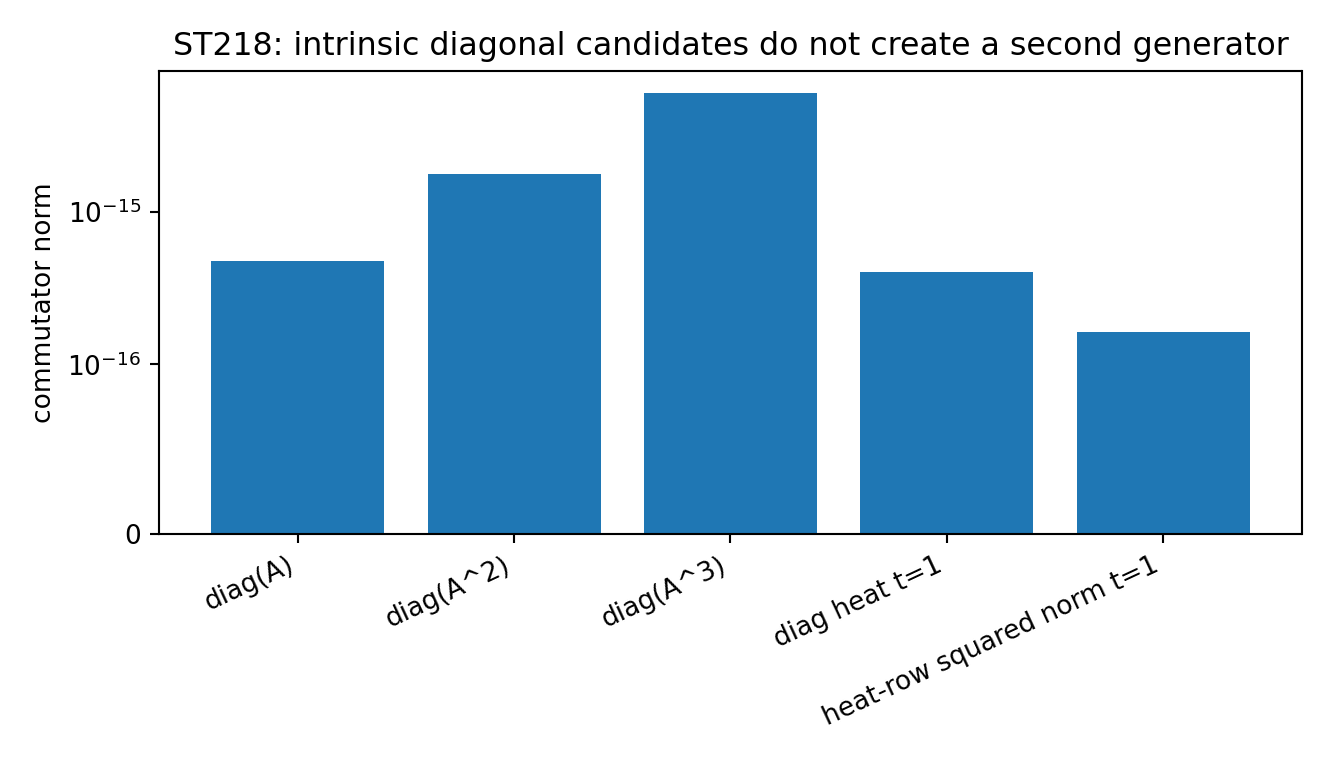
\includegraphics[width=.82\textwidth]{FIN_ST218_ST232_Figures/st218_noncommuting_no_go.png}
\caption{Every tested intrinsic diagonal candidate has zero commutator to numerical replay
precision. The theorem is stronger: the whole declared invariant algebra commutes.}
\end{figure}

\textbf{Interpretation.} A noncommuting layer is still possible, but it must carry something
not already present as an equivariant function of $A$: a transported state, orientation,
boundary, environment, or genuinely second operator. Calling such an object ``derived''
requires a separate provenance theorem.

\section{ST219: Blackwell order is preparation-relative}

For a finite preparation family, outcomes $x,y$ belong to the same minimal sufficient atom
exactly when their likelihood columns are proportional. If there are $m$ atoms, all
deterministic Blackwell quotients form the partition lattice $\Pi_m$, with rank numbers
$S(m,k)$ and Bell total $B_m$.

The audited families give:
\[
\begin{array}{c|c|c}
\text{preparation/instrument family}&m&B_m\\\hline
\text{localized vertices }\delta_0,\delta_1\text{ through }e^{-0.7A}&12&4{,}213{,}597\\
\text{thermal spectral preparations }\tau=.3,.8&7&877\\
\text{translation-averaged nonlinear-response location}&1&1\\
\text{orbit-averaged vertex preparations}&1&1
\end{array}
\]
The spectral count is exact from the seven spectral classes. The twelve vertex likelihood
ratios have a positive displayed separation in the frozen numerical instance; a future
transcendental interval proof is recommended.

\begin{figure}[H]
\centering
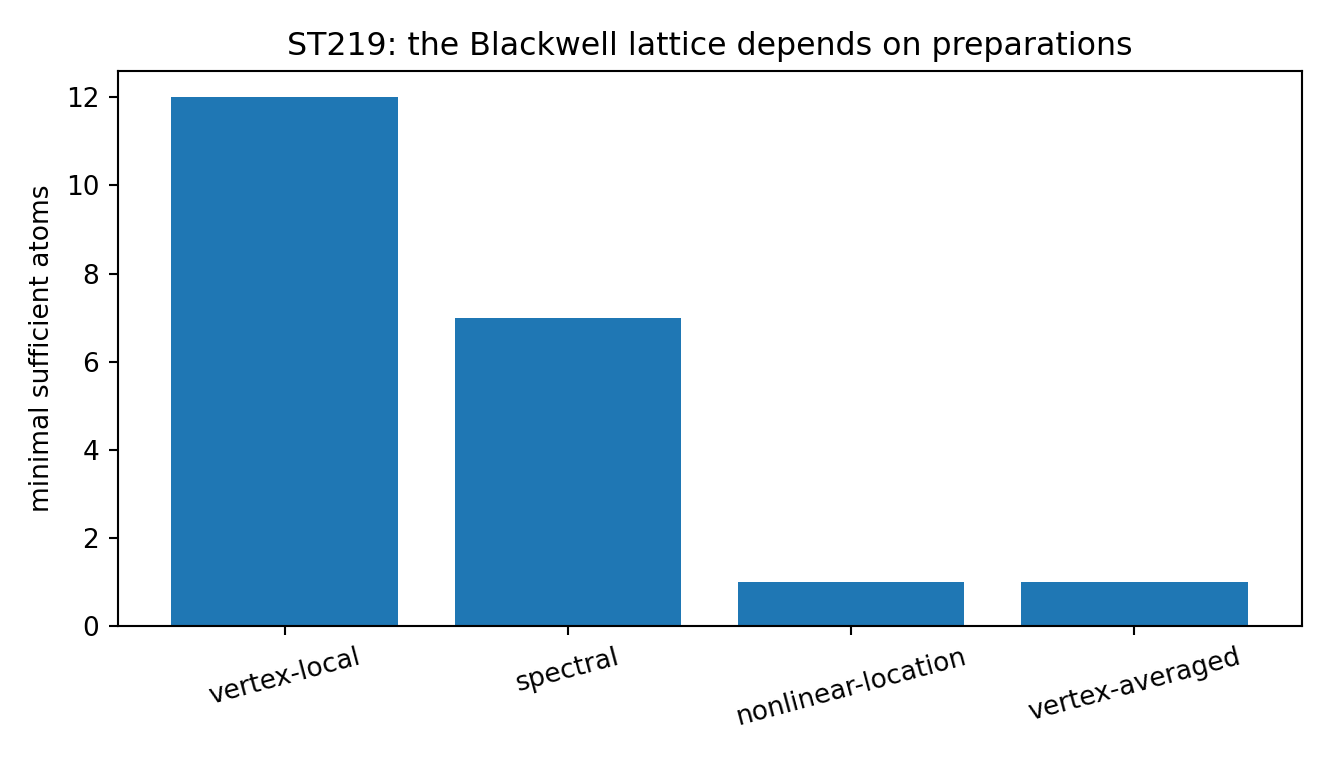
\includegraphics[width=.78\textwidth]{FIN_ST218_ST232_Figures/st219_blackwell_families.png}
\caption{The number of minimal sufficient atoms changes with the preparation family. A
Blackwell lattice is not an observer-independent ontology of $A$.}
\end{figure}

\section{ST220: invariant fluctuations cannot orient the cycle}

Let $G=D_{12}$ be the 24-element symmetry group generated by translations and reflection.
The Reynolds calculation gives seven orbits on ordered vertex pairs; therefore invariant
Gaussian covariances form the positive cone in a seven-dimensional distance-circulant
space. The only $G$-fixed vector is the constant vector, so the mean-zero sector has no
nonzero invariant drift.

\begin{theorem}[Invariant fluctuation selector no-go]
An invariant Gaussian or L\'evy triplet consists of a fixed drift, an invariant covariance,
and a jump measure constant on $G$-orbits. If the initial law and its coupling to the
dynamics are equivariant, every later law is invariant. Any equivariant branch readout has
equal probabilities on all twelve translated vertices, while reflection pairs the two
orientations. Such noise can realize a branch in one sample but cannot canonically label or
orient it.
\end{theorem}

This proves a complete no-go for the declared invariant stochastic class. It does not say
that asymmetric or state-conditioned noise cannot select; it says that the conditioning or
asymmetry is then the missing selector premise. QW-2191 is not discharged.

\section{ST221: all signed folds, not one selected branch}

Release 10.71 followed one branch. ST221 starts from every one of the sixty signed ST193
roots at $|\varepsilon|=.005$ and takes six outward pseudo-arclength steps. Every one of the
360 augmented hyperplanes passes outward Krawczyk inclusion.

\[
\begin{aligned}
N_{\rm seed}&=60, &N_{\rm certified}&=360/360,\\
\min \sigma_{\rm rank}&=2.5978389264\times10^{-3},&
\min\langle t_{n+1},t_n\rangle&=0.9998913243.
\end{aligned}
\]

\begin{figure}[H]
\centering
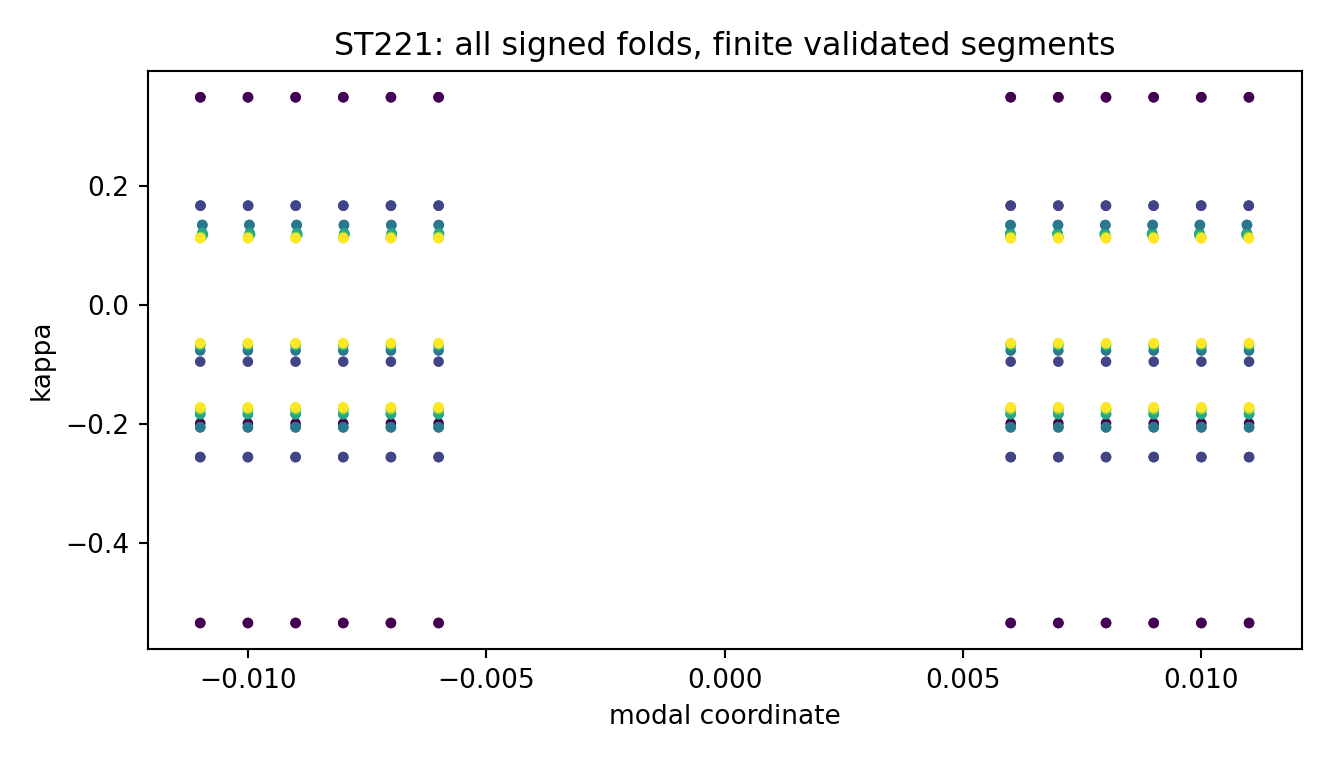
\includegraphics[width=.82\textwidth]{FIN_ST218_ST232_Figures/st221_all_fold_continuation.png}
\caption{Finite validated segments issued from all sixty signed seeds. Color denotes the
Fourier mode. No rank collision occurs at a certified point.}
\end{figure}

This is a substantial local atlas, not a proof of global connectivity, absence of distant
collisions, orbital stability, or particle physics.

\section{ST222: a non-diagonal negative-orientation recovery certificate}

The exact canonical Pauli probabilities are
\[
(p_I,p_X,p_Y,p_Z)=\left(\frac{2}{25},\frac{41}{100},\frac{29}{100},\frac{11}{50}\right),
\]
giving Bloch multipliers $(-.02,-.26,-.40)$ and negative determinant. Two noncommuting
rational rotations transform this into a visibly non-diagonal laboratory Bloch matrix with
off-diagonal Frobenius norm $0.37279648$.

Pauli twirling reduces the full CPTP recovery objective to
\[
\max_{q\in\Delta_4}\sum_i p_iq_i.
\]
The primal vertex $q_X=1$ attains $41/100$. The scalar dual $y=41/100$ satisfies
$y\ge p_i$ for every $i$, proving zero duality gap. Unitary covariance transports the
correction into the laboratory frame. Thus
\[
F_e^*=\frac{41}{100}.
\]
The theorem covers the two-sided rotated-Pauli class, not generic nonunital channels.

\section{ST223 and ST224: controlled selection and carrier naturality}

\subsection{A fixed-time dissipation bracket}

The reduced control law is
\[
x' = \pi+e^{-r\Delta t}(x-\pi),\qquad
\pi(b)=\frac{1}{1+11e^{-b}}.
\]
For one step, the audited relaxational entropy production is
\[
\Sigma=D(x\Vert\pi)-D(x'\Vert\pi)\ge0.
\]
Monotonicity of both the transition and $\Sigma$ away from $\pi$ permits an optimistic
interval-bin dynamic program. For eight steps in dimensionless time four, controls
$b\in\{1,2,3,4\}$ and $r\in\{.5,1\}$, and target $x\in[.59,.61]$, the result is
\[
0.3831118347\le \Sigma^*\le0.3931251756.
\]
The constructive schedule ends at $x=0.5930840189$. Field-switching work is deliberately
not included, so this is not yet the unrestricted thermodynamic optimum.

\subsection{The coordinate-free nonlinear invariant}

For a potential $V$, point $x$, and nonzero carrier direction $v$, define
\[
\mathcal I_{12}(V,x;v)=
\frac{D^{12}V_x[v,\ldots,v]}{11!\bigl(D^2V_x[v,v]\bigr)^6}.
\]

\begin{theorem}[Carrier naturality]
For every invertible linear carrier map $T$ and $V'=V\circ T^{-1}$,
\[
\mathcal I_{12}(V',Tx;Tv)=\mathcal I_{12}(V,x;v).
\]
Moreover $\mathcal I_{12}(V,x;cv)=\mathcal I_{12}(V,x;v)$ for every $c\ne0$.
\end{theorem}

The proof is the multilinear chain rule: each transported directional derivative is
unchanged, while direction rescaling multiplies numerator and denominator by $c^{12}$.
This makes the response ratio a genuine projective carrier invariant. It does not derive
the coupling $g$ or identify a physical carrier.

\section{ST225 and ST226: robust continuation and nonlocal sampling limits}

\subsection{Doubling the certified nuisance cube}

The previous global halfwidth was $2\times10^{-4}$. ST225 preserves the successful local
halfwidth $1.4285714\times10^{-5}$ while using a $28^3$ cover of the doubled cube:
\[
21{,}952/21{,}952\text{ boxes pass},\qquad
\min\text{ inclusion margin}=9.3607371\times10^{-4}.
\]

\begin{figure}[H]
\centering
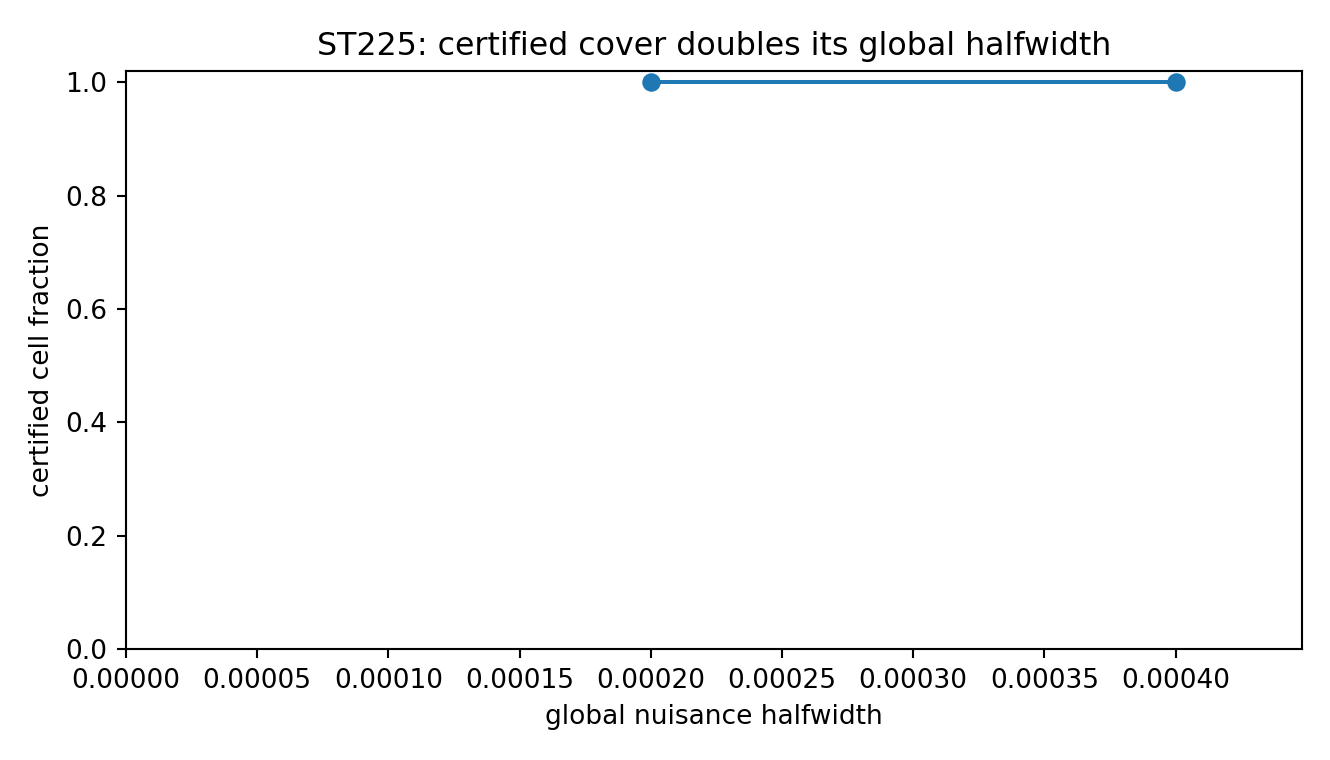
\includegraphics[width=.70\textwidth]{FIN_ST218_ST232_Figures/st225_cover_frontier.png}
\caption{The complete doubled nuisance cube is certified. The campaign then stops at its
declared finite computational boundary; this is not a maximal-domain theorem.}
\end{figure}

\subsection{Bounds valid for biased estimators}

For the least visible mode of the declared local Bernoulli model
\[
Y\sim\mathrm{Bernoulli}\left(\frac12+\sigma\theta\right),
\quad |\theta|\le.2,
\quad \sigma=2^{-12},
\]
Le Cam's two-point method and Pinsker give
\[
\inf_{\widehat\theta}\sup_\theta
\mathbb E_\theta(\widehat\theta-\theta)^2
\ge \frac{\delta^2}{2}
\left(1-\sqrt{\frac{nD(P_\delta\Vert P_{-\delta})}{2}}\right)_+.
\]
This applies to biased and unbiased estimators. If additionally $|b'(\theta)|\le\beta<1$,
biased Cram\'er--Rao gives
\[
\mathrm{MSE}\ge\frac{(1-\beta)^2}{nI(\theta)}.
\]

\begin{figure}[H]
\centering
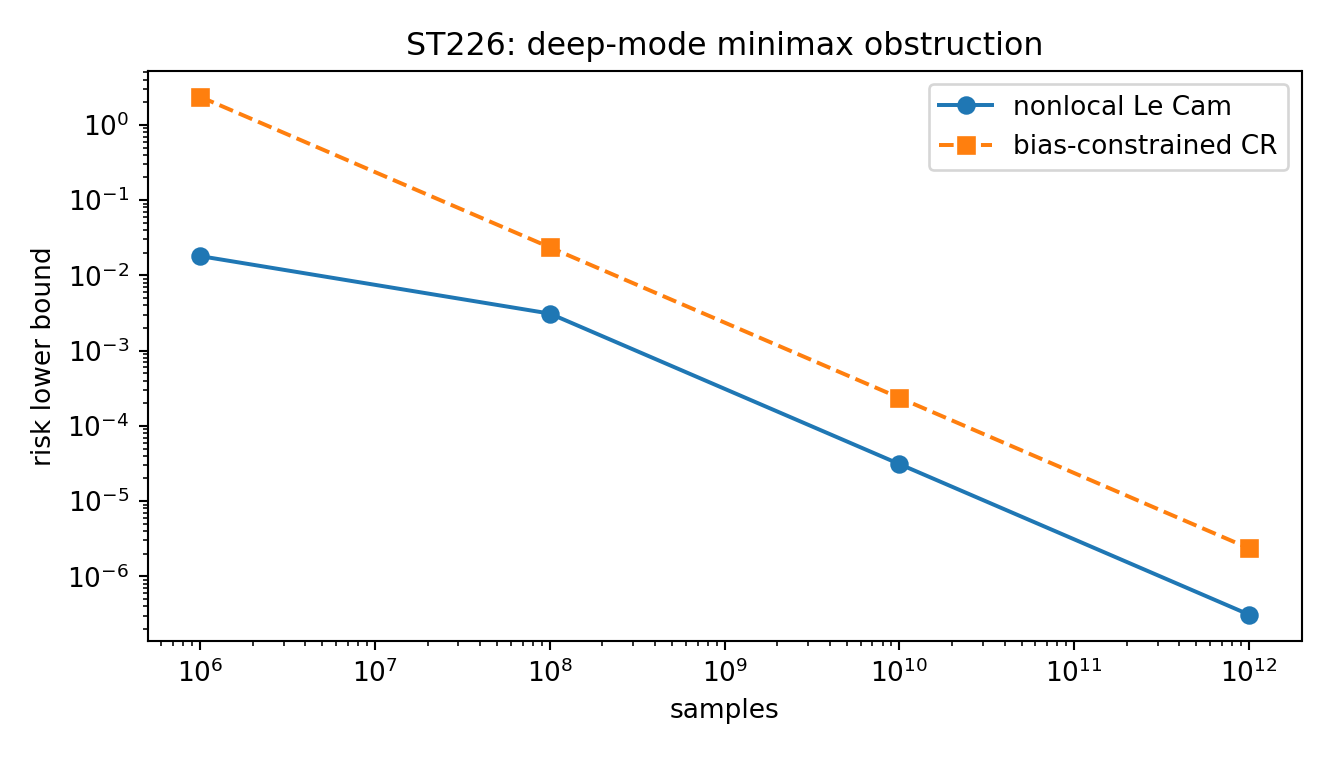
\includegraphics[width=.78\textwidth]{FIN_ST218_ST232_Figures/st226_minimax_bounds.png}
\caption{Nonlocal Le Cam and bias-constrained local bounds for the depth-twelve mode.}
\end{figure}

\section{ST227 and ST228: uniqueness with a gap and a sharper HMM rate}

\subsection{Nearest joint factors}

Traceless Hermitian qubit involutions are $X=\bm n\cdot\bm\sigma$ and
$Z=\bm m\cdot\bm\sigma$. Exact anticommutation is $\bm n\cdot\bm m=0$; hence
$Q=[\bm n,\bm m]\in V_2(\R^3)$. The nearest joint-factor problem becomes rectangular
Procrustes:
\[
\max_{Q^TQ=I_2}\Tr(Q^TB).
\]

\begin{theorem}[Gap-conditioned uniqueness]
If $B$ has full column rank, the unique global solution is the rectangular polar factor
\[
Q_*=B(B^TB)^{-1/2}.
\]
\end{theorem}

For the declared target, $\lambda_{\min}(B^TB)=0.4161946708$ and the constraint error is
$2.49\times10^{-16}$. The ST212 circle occurs exactly at the rank-one boundary where the
premise fails.

\subsection{Exact belief cylinders}

Exact rational forward recursion was extended from length 12 to all $2^{16}=65{,}536$
observation cylinders. Outward integer-square-root summation gives
\[
0.6898819929\le R_{1/2}\le0.8198470893.
\]
The width is $\log(8)/16=0.1299650964$, exactly $75\%$ of the preceding width. The
calculation certifies the Hellinger point $s=1/2$, not the optimized Chernoff exponent.

\section{ST229: reset is possible as reversible information transfer}

Let two identical 16-level registers have total Hamiltonian
\[
H_{\rm tot}=H\otimes I+I\otimes H.
\]
The four corresponding qubit-pair SWAPs do not individually commute with $H_{\rm tot}$ in
the frozen encoding; their commutator norms lie between $2.34$ and $2.73$. Nevertheless,
their product is the exact global register SWAP $S$, and
\[
[H_{\rm tot},S]=0.
\]
For a prepared blank state $\beta$,
\[
S(\rho\otimes\beta)S^\dagger=\beta\otimes\rho.
\]
Thus the first register is reset and final total energy is conserved. The information has
moved to the second register. It has not disappeared. This exact construction cleanly
separates three notions:
\[
\text{pointwise energy conservation}
\ne\text{final energy conservation}
\ne\text{information erasure}.
\]
The blank ancilla, identical Hamiltonian, exact pulses, and timing are operational resources.

\section{ST230: four internal geometries are not one metric}

For vertices $i,j$, the report compares
\begin{align*}
D_t(i,j)&=\|(e_i-e_j)^Te^{-tA}\|_2,\\
R^{1/2}(i,j)&=\bigl((e_i-e_j)^TA^+(e_i-e_j)\bigr)^{1/2},\\
H_t(i,j)&=\left(\sum_x(\sqrt{C_t(i,x)}-\sqrt{C_t(j,x)})^2\right)^{1/2},\\
P_1(i,j)&=\|(e_i-e_j)^TP_{\lambda_1}\|_2.
\end{align*}
The Hellinger embedding has the Fisher--Rao metric as its local quadratic form; it is not
being identified with a global Fisher geodesic distance.

\begin{figure}[H]
\centering
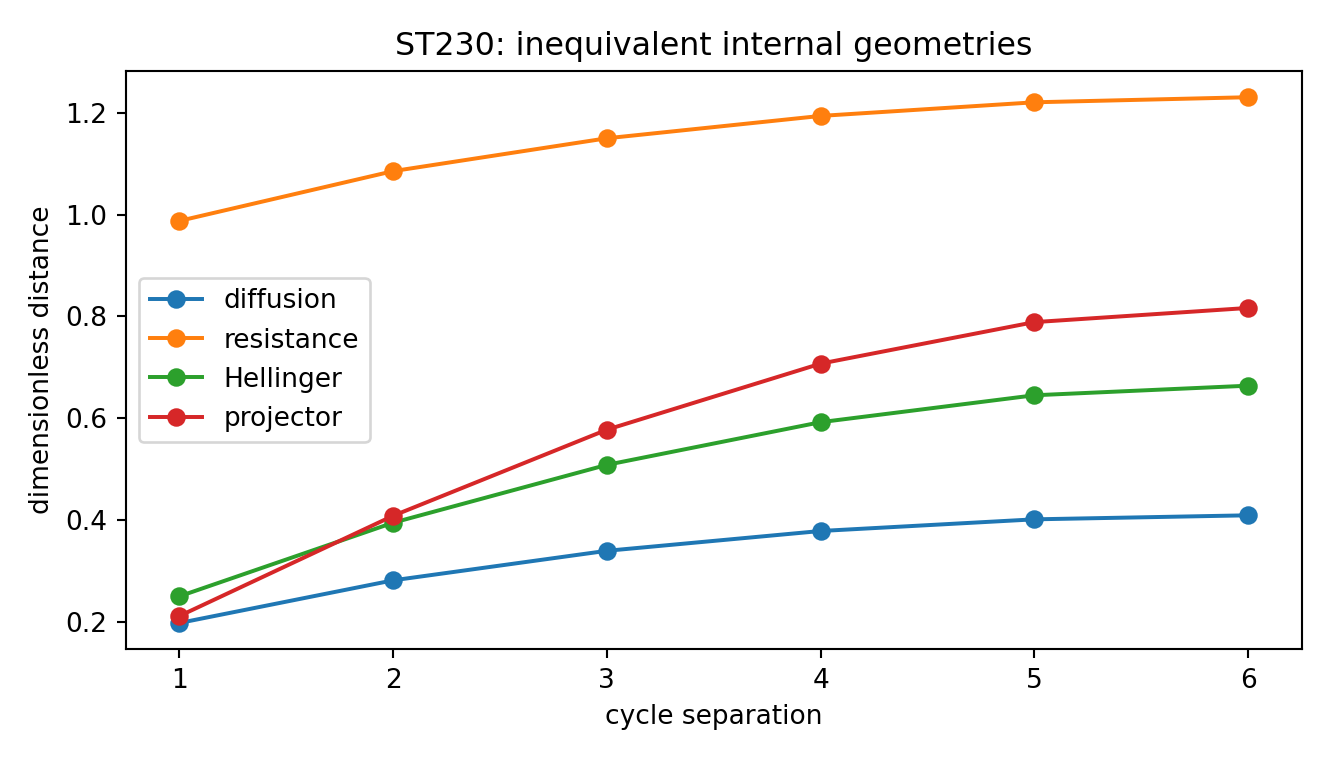
\includegraphics[width=.82\textwidth]{FIN_ST218_ST232_Figures/st230_metric_atlas.png}
\caption{All four metrics respect cyclic separation but have nonconstant pairwise ratios.
Similarity of shape is not equality.}
\end{figure}

At $t=1$, $D_t/R^{1/2}$ ranges from $0.2002$ to $0.3326$, while $D_t/P_1$ ranges from
$0.5012$ to $0.9355$. Therefore no one scalar identifies these geometries. ST215's
long-time result remains valid: rescaled diffusion converges specifically to the first
spectral-projector chord.

\section{ST231: exact refinement and the scale nonuniqueness theorem}

Let
\[
L_2=\begin{pmatrix}1&-1\\-1&1\end{pmatrix},\qquad
u=\frac{1}{\sqrt2}(1,1)^T,
\]
and define
\[
A_{24}=A_{12}\otimes I_2+\mu I_{12}\otimes L_2,
\qquad Re_i=e_i\otimes u,
\qquad \mu\ge0.
\]

\begin{theorem}[Diffusion-preserving two-child refinement]
For every $\mu\ge0$,
\[
A_{24}R=RA_{12},\qquad
e^{-tA_{24}}R=Re^{-tA_{12}}.
\]
Because $R$ is an isometry, every coarse diffusion distance is preserved exactly after
lifting.
\end{theorem}

The proof is immediate from $L_2u=0$ and functional calculus. Numerical replay for
$\mu\in\{.2,1,5,20\}$ and three times has maximum distance error
$3.22\times10^{-15}$.

\begin{figure}[H]
\centering
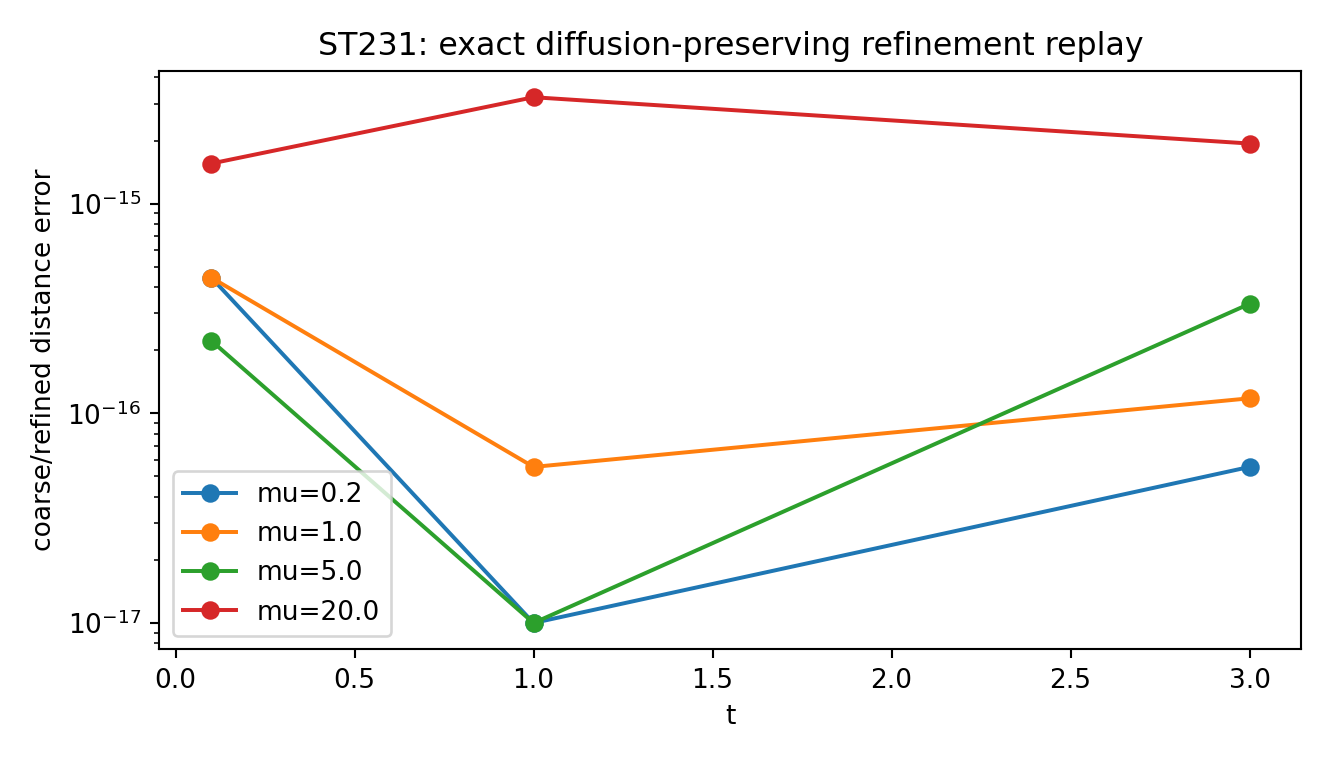
\includegraphics[width=.78\textwidth]{FIN_ST218_ST232_Figures/st231_refinement.png}
\caption{Coarse/refined distance mismatch is at roundoff level for four different fiber
rates. The continuous family is the important result.}
\end{figure}

This construction formalizes one version of ``seeing a lower scale through a developed
layer'': the coarse observable sector is an invariant isometric subspace of a finer operator.
But $\mu$ is arbitrary. Neither the strict coarse geometry nor the intertwining law chooses
a child time, length ratio, Planck scale, or unique $Z_{24}$ kernel. The object is an exact
operator refinement, not yet a physical fractal hierarchy.

\section{ST232 and the physical boundary}

\Blocked{} No external event record, independent registrar, calibration artifact, or
laboratory attestation was supplied. A local program can verify syntax, hashes, interval
certificates, and mathematical implications. It cannot create evidence that an independent
apparatus interacted with nature. ST232 therefore performs no synthetic substitute.

\section{What changed in the theory}

The current local mathematical picture can now be stated more precisely.

\begin{itemize}
\item The strict operator supports unitary, heat, Green, wave, and response channels, but a
single common functional calculus cannot encode their ordered layer history.
\item Invariant stochasticity explains random realization without explaining canonical
orientation. Symmetry is a reservoir of equivalent possibilities, not itself positive
feedback or a selector.
\item Nonlinear information can be transported through carrier changes by a precise
projective invariant $\mathcal I_{12}$.
\item Coarse diffusion geometry can survive exact refinement. This supports a rigorous
multilayer interpretation at the operator level.
\item The same refinement theorem proves a scale obstruction: many finer dynamics have the
same coarse geometry.
\item Reset under final energy conservation is possible by reversible transfer to an
ancilla, clarifying the operational meaning of information preservation.
\end{itemize}

The ontology guardrail remains unchanged: within FIN, the nadsoliton is the primordial
fractal information in a solitonic state; no separate informational substrate is inserted
below it. The present mathematics neither verifies nor falsifies that ontology as a claim
about nature. It determines what follows from the declared operators and what still requires
an additional axiom or experiment.

\section{Recommended programs ST233--ST247}

\small
\begin{longtable}{>{\bfseries}p{0.10\textwidth}p{0.08\textwidth}p{0.73\textwidth}}
\toprule
Program & Rank & Study\\
\midrule
\endhead
ST233&1&Introduce exactly one typed second operator; audit strict provenance, noncommutation, and schedule identifiability.\\
ST234&2&Certify the twelve localized vertex likelihood classes by transcendental interval arithmetic.\\
ST235&3&Classify state-conditioned equivariant noise and locate exactly where conditioning becomes a selector premise.\\
ST236&4&Adaptively extend all ST221 branches and build a certified component/collision graph.\\
ST237&5&Solve one genuinely nonunital negative-orientation qubit recovery SDP with rational primal--dual witnesses.\\
ST238&6&Upgrade ST223 to verified continuous control, including switching work.\\
ST239&7&Extend $\mathcal I_{12}$ naturality to nonlinear carrier charts and response bundles.\\
ST240&8&Extend the ST225 nuisance cube until a certified fold boundary or an explicit resource stop.\\
ST241&9&Derive sharp simultaneous-mode minimax constants under correlated counts.\\
ST242&10&Generalize polar joint-factor uniqueness to higher-dimensional balanced Clifford pairs.\\
ST243&11&Optimize the observed-HMM Chernoff parameter with certified belief-space transfer bounds.\\
ST244&12&Complete work--information bookkeeping for the reversible reset and blank-ancilla preparation.\\
ST245&13&Classify all finite-fiber diffusion-preserving refinements and their nonuniqueness moduli.\\
ST246&14&Test spectral-dimension flow under repeated exact refinements without assigning physical length.\\
ST247&15&Resume external validation only with a genuine independently registered event package.\\
\bottomrule
\end{longtable}
\normalsize

ST233 has the greatest foundational leverage. It must not merely rename a basis choice as a
strict consequence. A successful candidate needs a typed source, a transformation law, a
proof that it is not $f(A)$, and a demonstration that its noncommutation leaves a measurable
schedule invariant. ST245--ST246 most directly continue the user's intuition about developed
fractal layers while respecting the current absence of a physical length unit.

\section{Reproducibility and provenance}

The executable release contains:
\begin{itemize}
\item \texttt{fin\_st218\_st232\_research.py};
\item \texttt{test\_fin\_st218\_st232.py};
\item one complete result ledger, one summary CSV, and fifteen specialized JSON packets;
\item seven generated figures;
\item this source report and compiled PDF;
\item the English Release 10.72 description and SHA-256 manifest.
\end{itemize}

The local validation suite contains 52 live and serialized assertions. The expensive
$28^3$ Krawczyk campaign is serialized with hashes rather than rerun inside the lightweight
test suite; the main research script reproduces it. Seed \texttt{20260812} controls only
finite randomized replays, not exact algebraic or interval theorems.

The principal internal sources are the Release 10.69--10.71 result ledgers and executable
scripts, the current root \texttt{AGENTS.md}, the kernel split/provenance packets
\texttt{K1}, \texttt{K2}, \texttt{F2}, \texttt{F3}, \texttt{S2}, and
\texttt{SUMMARY\_GROK.md}. Claims inherited from earlier programs are explicitly labeled as
repository results; all new numerical values in this report are emitted by the Release
10.72 ledger.

\section{Final verdict}

\begin{quote}
\textbf{The current FIN strict operator generates a rich family of compatible dynamics and
an exactly refinable dimensionless geometry, but it does not generate the extra
noncommuting information needed to identify a fractal layer history or a canonical
orientation. Exact refinement is possible, yet continuously nonunique. The missing bridge
is therefore no longer merely ``more layers'': it is a sourced second typed object plus an
operational dimensional calibration.}
\end{quote}

This verdict is compatible with further FIN research. It is not a claim that FIN is a
physical Theory of Everything.

\end{document}
